\chapter{数学基础-DEMO}
\label{chap:math_regression}

AI实在是一个多学科综合性应用,涉及到的理论不仅多而且深。限于笔者知识水平以及篇幅要求,不会对此进行长篇巨幅地解释。


\section{向量运算}
单独的一个数字,称为\emph{标量}(scalar),而向量通常用数组的形式表示。一个\emph{向量}就是一列(行)数字:
\begin{equation}
x=[x_1 x_2 \dots x_n],
x=\left[\begin{array}{c} x_1\\x_2\\\dots\\x_n\end{array}\right]
\label{part2_vector_form}
\end{equation}
\ \\
向量是一种带方向指示性的量,代表空间中的一个点。一维向量$\vec{a}=\left[4\right]$代表a点在原点右侧距离为4的位置。
而二维向量$\vec{b}=\left[3\ 4\right]$就代表了在第一象限坐标(3,4)有一个点b。所以,向量是一个方向性的偏移量。
\emph{向量}可以在坐标系中自由平移,选定一个起点就确定了它的终点。

\begin{center} \begin{tikzpicture}
\node[circle,draw,black,scale=0.2] (A) at (1,2) {};
\node[circle,draw,black,scale=0.2] (B) at (3,4) {};
\draw[arrow]
    (A)node[below]{A起点}--(B)node[above]{B终点};
\end{tikzpicture}\end{center} 

向量支持的运算有\emph{内积}(点乘)和\emph{外积}(叉乘)运算,以及加减运算。
向量A、B的运算过程,设$\vec{A} = (a1,  a2,  a3), \vec{B} = (b1,  b2,  b3)$

\begin{itemize}
\item[1.] 点乘,结果是一个标量:$A \cdot B = a1*b1 + a2*b2 + a3*b3$
\item[2.] 叉乘,结果还是个向量:$A \times B = (a2*b3 - a3*b2, a3*b1 - a1*b3, a1*b2 - a2*b1)$
\item[3.] 标量,用于每一个元素:$A + 2 = (a1+2, a2+2, a3+2)$
\end{itemize}

\noindent
通常使用\emph{数组}来表示向量,但这样扩展性不够好。咱们使用Java面向对象的方法,把数组和函数封装进一个向量类型里面去。定义一个Vector类,如\figref{fig:part2_math_vector}:

\begin{figure}[!htb]
\begin{center}\begin{tikzpicture}
\umlclass[y=-3]{InVector}{
    array : int[] 
}{
    add(v : InVector) : InVector \\
    sub(v : InVector) : InVector \\
    dot(v : InVector) : int \\
    cross(v : InVector) : IntVector
}
\end{tikzpicture}\end{center}
\caption{类图:IntVector}
\label{fig:part2_math_vector}
\end{figure}

\begin{lstlisting}[language=Java]
public IntVector(int... array) {
    this.array = array;
}

public IntVector add(IntVector vector) {
    foreach(this.array, vector.array, (a,b)->a+b);
    return this;
}

public int dot(IntVector vector) {
    return foreach(this.array, vector.array, (a,b)->a*b);
}
\end{lstlisting}

如上代码,构造函数用到了可变参数,你可以理解成一个\lstinline{int[]}。在编译的时候,Java会自动地把函数声明和调用代码都转换成数组。
\emph{add}运算返回\lstinline{this},用来支持链式运算:$v1.add(v2).add(v3)\dots$。容易看出,
\emph{add}和\emph{dot}运算,是对应元素相加、相乘的过程。
使用\emph{foreach}从相加的2个向量中,逐个地取出数据并执行$\lambda$操作。

\begin{lstlisting}[language=Java,caption=叉乘运算]
public IntVector cross(IntVector vector) {
    int[] v1 = this.array;
    int[] v2 = vector.array;

    int length = vector.array.length;
    if (length == 2) {
        return new IntVector(v1[0]*v2[1]-v1[1]*v2[0]);
    }

    int[] result = IntStream.range(0, length).map(
        i->v1[(i+1)%length]*v2[(i+2)%length] -v1[(i+2)%length]*v2[(i+1)%length]
    ).toArray();

    return new IntVector(result);
}

// sum用于dot运算
private static int foreach(int[] src, int[] dst, IntBinaryOperator op) {
    int sum = 0;
    for (int i = 0; i < src.length; i++) {
        src[i] = op.applyAsInt(src[i], dst[i]);
        sum += src[i];
    }
    return sum;
}
\end{lstlisting}

以上,仅仅只能处理int类型的向量。
结合IntVector的实现代码,相信大家也能理解实数类型的向量。
也许你也意识到,使用\emph{add}太麻烦了,但Java目前还不支持运算符重载。
如果确实想使用,可以借助\emph{Java-OO开源插件}\footnote{一种使用APT在编译过程中替换运算符为相应函数的方法。}
\vspace{0.3cm}

\begin{lstlisting}[language=Java, caption=运算符重载]
@Test
public void add_operator_override() {
    IntVector a = new IntVector(1,2,3);
    IntVector b = new IntVector(10,20,30);

    IntVector c = a + b; // 看上去运算符重载了
    int[] expected = new int[]{11, 22, 33};

    assertArrayEquals(expected, c.array);
    assertEquals(new IntVector(expected), c);
}
\end{lstlisting}

实际上,很少有自己实现的,并且也较难保障准确性和稳定性。开源的ND4J作为DL4J的张量计算库,提供了丰富的运算接口,支持几乎所有的数学操作,相当于Python界的numpy。以下\coderef{code:part2_math_dl4j}

\begin{lstlisting}[language=Java,caption={dl4j例子},label=code:part2_math_dl4j]
INDArray vec1 = Nd4j.create(new float[]{1,2,3});

// vector add
INDArray vec2 = Nd4j.create(new float[]{10,20,30});

// [[11.0000, 22.0000, 33.0000]]
System.out.println(vec1.add(vec2));

// scalar add
INDArray vec3 = vec1.add(10);

// [[11.0000, 12.0000, 13.0000]]
System.out.println(vec3);
\end{lstlisting}

ND4J在开源、分布式、支持GPU的库内,为Java带来了符合直觉的,类似Python编程人员所用的科学计算工具。
它具有:
\begin{itemize}
\item[1.] 多用途多维数组对象
\item[2.] 多平台功能,包括GPU
\item[3.] 线性代数和信号处理功能
\end{itemize}

\noindent
本节之后都将使用ND4J来演示算法,有兴趣的同学可以研究它的实现代码。

\section{矩阵运算}

矩阵是一个$m \times n$个数组成的m行n列的矩形表格。
特别地,向量可以看作矩阵的特殊形式。
对于$1 \times n$或$n \times 1$的矩阵,就是一个行向量或列向量。
实际上,矩阵的\emph{加法/减法}运算,也可适用于向量。
尽管矩阵是多维度数据,却很少采用多维数组表示。
如果\emph{向量}和\emph{矩阵}都使用一维数组表示的话,\emph{add}运算当然可以用与矩阵。

\vspace{0.3cm}\noindent
对于这样一个数组: \lstinline|int[] numbers={1,2,3,4,5,6}|。
\begin{itemize}
\item[1.] 可能是一个$1 \times 6$的矩阵,或是一个向量。
\item[2.] 可能是一个$2 \times 3$的矩阵
\item[3.] 可能是一个$3 \times 2$的矩阵
\end{itemize}

\begin{figure}[!htb]
\begin{center}\begin{tikzpicture}
\umlclass[y=-3]{IntNDArray}{
    array : int[] \\
    shape : int[]
}{
    add(v : IntNDArray) : IntNDArray \\
    mul(v : IntNDArray) : IntNDArray \\
    rank(): int \\
    isVector(): boolean
}
\label{fig:part2_math_matrix}
\end{tikzpicture}\end{center}
\caption{类图:IntNDArray}
\end{figure}

为了让IntVector升级为IntNDArray,势必要加入维度信息才行,记为\emph{shape}。而矩阵只有2个维度,如果不考虑更多维度的情况下,
使用\lstinline|int[2]|就可以。但你立即就会认识到,改成\lstinline|int[]|有更好的可扩展性。
使用\emph{IntNDArray}创建向量就是创建$1 \times n$或$n \times 1$的矩阵。

\begin{lstlisting}[language=Java,caption={创建NDArray}]
int[] array;
int[] shape;

// 默认:1 x n
public IntNDArray(int... array) {
    this.array = array;
    this.shape = new int[]{1, array.length};
}

// 可以把1x6转换成2x3或者3X2的矩阵
public IntNDArray reshape(int[] shape) {
    this.shape = shape;
    return this;
}
\end{lstlisting}

根据数学定义,只有当矩阵A的列数等于矩阵B的行数时,A与B才可以相乘。乘积C的第m行第n列的元素等于矩阵A的第m行的元素与矩阵B的第n列对应元素乘积之和。

\begin{equation}
c_{ij}= \sum_{k=1}^pa_{ik}*b_{kj}
\end{equation}
其中,A为m $\times$ p的矩阵,B为p $\times$ n,结果为mxn的矩阵C。
相应地,实现算法如下:

\begin{lstlisting}[language=Java,caption={矩阵乘法}]
public IntNDArray mul(IntNDArray ndArray) {
    final int ROWS = this.shape[0];
    final int COLS = ndArray.shape[1];

    int[] shape = new int[]{ROWS, COLS};
    int[] data = new int[ROWS*COLS];

    for(int i=0; i<ROWS; i++) {
        for (int j=0; j<COLS; j++) {
            for (int k=0; k<ndArray.shape[0]; k++) {
                int a_i_k = this.array[i*this.shape[1]+k];
                int b_k_j = ndArray.array[k*ndArray.shape[1]+j];
                data[i*COLS+j] += a_i_k * b_k_j;
            }
        }
    }
    return new IntNDArray(data).reshape(shape);
}
\end{lstlisting}

现在,我们就可以用一维数组记录矩阵了,不管维度如何变化reshape之后不需要变更array的内容。
对于\emph{向量}的点乘和叉乘,也可以借助\emph{矩阵}处理。
\emph{点乘}比较容易解决,但\emph{叉乘}需要\emph{反对称}矩阵(anti-symmetric)辅助才能计算出结果。
不过\emph{叉乘}主要应用于几何和动量计算,在此就不再详细解释。

\vspace{0.3cm}\noindent
以下代码是ND4J的矩阵示例:
\begin{lstlisting}[language=Java]
INDArray v1 = Nd4j.create(new float[]{1,2,3}).reshape(1,3);
INDArray v2 = Nd4j.create(new float[]{10,20,30}).reshape(3,1);
System.out.printf("v1v2=[%s]\n", v1.mmul(v2));
\end{lstlisting}


\section{梯度下降}
在机器学习里,梯度下降虽然不是什么高深的算法,但它却是机器学习的关键。经常会用到梯度下降法来进行训练,常见的有:
批量梯度下降法BGD,随机梯度下降法SGD,小批量梯度下降法MBGD。

\begin{figure}[!htb]
\centerline{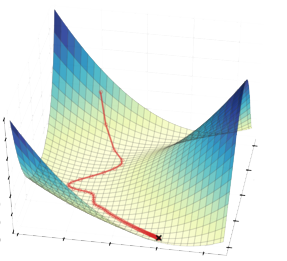
\includegraphics[width=.2\figwidth]{images/sgd.png}}
\label{fig:part2_math_sgd}
\caption{梯度下降}
\end{figure}

梯度是方向上升/下降最快的方向,它的幅值代表陡峭的程度。
所以,在最小值的地方,曲面轮廓几乎是平坦的,理论上最小值是梯度为0。
但事实上,我们又可能无法达到最小值,只能在最小值附近的平坦区域来回震荡。
当在这个区域震荡时,损失(Loss)值几乎是我们能达到的最小值了,并且不会有很大的变化,因此我们是在真实的最小值附近跳动。
通常,当损失值在预定的数字内没有改善的时候就会停止迭代,例如10次或者20次迭代。
当这种情况发生时,就说训练已经收敛了,或者说收敛已经完成了。

\subsection{BGD}
使用BGD(Batch Gradient Descent,批量梯度下降),在目标函数为凸函数时,虽然可以找到全局最优解,
但收敛速度慢,需要用到全部数据,因此内存消耗也大。因此,BGD不适用于大数据集。
其公式如下:

\noindent
$$\boldsymbol{W} \leftarrow \boldsymbol{W}-\eta \frac{\partial \boldsymbol{L}}{\partial \boldsymbol{W}}$$

\noindent
如公式所示,BGD的策略就是朝着当前所在位置的坡度最大的方向前进。
但它也有缺点,它在面对峡谷型函数时,效率会变得很低,呈现出震荡的姿态。

\subsection{SGD}
而SGD相当于BGD的升级版。SGD被称为随机梯度下降(Stochastic Gradient Desccent)。
正如它的名字所说,它首先通过mini-batch学习,
意思就是从训练数据中随机选择一部分数据(称为mini-batch),
将这些mini-batch作为对象,使用梯度法进行学习。
其代码如下所示:


\begin{lstlisting}[language=java]
	MultiLayerConfiguration conf = new NeuralNetConfiguration.Builder()
        .weightInit(WeightInit.XAVIER)
        .activation("relu")
        .optimizationAlgo(OptimizationAlgorithm.STOCHASTIC_GRADIENT_DESCENT)
        .updater(new Sgd(0.05))
        // ... other hyperparameters
        .list()
        .backprop(true)
        .build();
\end{lstlisting}


\subsection{Momentum}
Momentum也是一种常见的优化算法,也被称为SGD with Momentum。
恰如其名,它为了抑制SGD的震荡,在梯度下降过程中加入惯性。
简单来说,它就是在梯度越陡时,下降越快。较平缓时,下降较慢。
其公式如下:

$$\boldsymbol{v} \leftarrow \alpha \boldsymbol{v}-\eta \frac{\partial \boldsymbol{L}}{\partial \boldsymbol{W}}$$

$$\boldsymbol{W} \leftarrow \boldsymbol{W}+\boldsymbol{v}$$

\noindent
如上式所示,$\boldsymbol{W}$表示要更新的权重参数,$\frac{\partial L}{\partial \boldsymbol{W}}$
表示损失函数关于$\boldsymbol{W}$的梯度,$\eta$表示学习率。
而$\boldsymbol{v}$这一变量便是用来模拟惯性的。
其通过在SGD的基础上引入一阶动量,
这代表着现在下降方向不仅由当前点的梯度方向决定,而且由此前累积的下降方向决定。 


\begin{lstlisting}[language=java]
	MultiLayerConfiguration conf = new NeuralNetConfiguration.Builder()
        .weightInit(WeightInit.XAVIER)
        .activation("relu")
        .optimizationAlgo(OptimizationAlgorithm.STOCHASTIC_GRADIENT_DESCENT)
        .updater(new Nesterovs(0.05))
        // ... other hyperparameters
        .list()
        .backprop(true)
        .build();
\end{lstlisting}

\noindent
Momentum的更新路径就如同小球在碗中滚动一样。
与SGD相比,其大大缓解了震荡问题,原因就是它加入的一阶动量。
即使在某一方向“受力”很小,但因为其一直在同一方向受力,
所以它会朝着同一方向有一定的加速。
通俗地讲,就是它所加入的惯性,抵消了试图改变它的力。

\subsection{AdaGrad}
在梯度下降中,学习率的值很重要(记为$\eta$),
而在学习率的相关研究中,有一种被称为\textbf{学习率衰减}(learning rate decay)的方法,
随着机器学习的过程,使学习率逐渐减小。
它具体表现为,在一开始与其他方法类似,进行参数学习,
但在学习的过程中,当准确率越来越高时,便减少学习率。
其公式如下:
$$\boldsymbol{h} \leftarrow \boldsymbol{h}+\frac{\partial \boldsymbol{L}}{\partial \boldsymbol{W}} \odot \frac{\partial \boldsymbol{L}}{\partial \boldsymbol{W}}$$

$$\boldsymbol{W} \leftarrow \boldsymbol{W}-\eta \frac{1}{\sqrt{\boldsymbol{h}}} \frac{\partial \boldsymbol{L}}{\partial \boldsymbol{W}}$$

如公式所示,AdaGrad会为参数的每个元素适当地调整学习率,
与此同时进行参数的学习。AdaGrad的公式比起之前的,
新出现了一个变量$\boldsymbol{h}$,它代表着之前所有梯度值的平方和,
在更新参数时,通过乘以$\frac{1}{\sqrt{\boldsymbol{h}}}$,
AdaGrad便可以为每个元素调整适宜它的学习率。其代码如下所示:

\begin{lstlisting}[language=java]
	MultiLayerConfiguration conf = new NeuralNetConfiguration.Builder()
        .weightInit(WeightInit.XAVIER)
        .activation("relu")
        .optimizationAlgo(OptimizationAlgorithm.STOCHASTIC_GRADIENT_DESCENT)
        .updater(new AdaGrad(0.05))
        // ... other hyperparameters
        .list()
        .backprop(true)
        .build();
\end{lstlisting}
AdaGrad比起Momentum更好地抑制了SGD的震荡,函数的取值高效地向着最小值移动。
刚开始时,也许还会有些震荡,但越接近最小值,几乎是呈直线般向着目标前进。

\subsection{Adam}

\begin{lstlisting}[language=java]
	MultiLayerConfiguration conf = new NeuralNetConfiguration.Builder()
        .weightInit(WeightInit.XAVIER)
        .activation("relu")
        .optimizationAlgo(OptimizationAlgorithm.STOCHASTIC_GRADIENT_DESCENT)
        .updater(new Adam(0.05))
        // ... other hyperparameters
        .list()
        .backprop(true)
        .build();
\end{lstlisting}




\section{概率分布}

\section{损失函数}
在机器学习中,机器的学习需要某个指标来表示现在的状态,然后,以这个指标为基准,寻找最优权重参数。
而在机器学习中所用的指标便被称为\emph{损失函数}(loss function)。
对于损失函数,我们主要使用均方误差和交叉熵误差。

首先,我们介绍一种常用的函数,\emph{交叉熵误差}(cross entropy error)。
\begin{equation}
    E = - \sum _ { k } t _ { k } \log y _ { k }
    \label{part2_cross_entropy_error_1}
\end{equation}

在上式中,$y_{k}$代表着机器学习的输出,log表示以e为底数的自然对数($log_{e}$)。
$t_{k}$代表着正确解标签,仅当解标签为正确时,$t_{k}$的索引才为1。其余情况都为0。
因此,E所代表的实际为解标签为正确时所输出的自然对数。

%交叉熵误差的图像

如上图所示,当输出结果$y_{k}$越发趋向于1.0时,得到的E越发增大而趋向于0。
交叉熵误差通过E所表示的负值,来表明该权重参数与正确结果之间的偏差程度。

下面,我们用代码来实现交叉熵误差:
%代码
\begin{lstlisting}[language=Java,caption={交叉熵误差}]
\end{lstlisting}

%代码分析

%实际运行

\ \\
下面我们介绍另一种,在损失函数中最有名的\emph{均方误差}(mean squared error)。
它的公式如下所示:

\begin{equation}
    E = \frac { 1 } { 2 } \sum _ { k } \left( y _ { k } - t _ { k } \right) ^ { 2 }
    \label{part2_cross_entropy_error_2}
\end{equation}

在上式中k表示着数据处于哪一个维度,$t_{k}$表示着各维度的监督数据。通常情况下,
监督数据仅将正确解标签表示为1,而其他非正确解则表示为0。
而机器学习输出的结果$y_{k}$,则是会在各个维度都显示该维度是正确解标签的可能性。
均方误差通过计算机器学习的输出和正确解监督数据的各个元素之差的平方,再求总和。
从而得到该权重参数的输出结果与正确结果之间的偏差。

%代码
\begin{lstlisting}[language=Java,caption={均方误差}]
\end{lstlisting}

%代码分析

%实际运行

\section{拟合算法}

很多时候,我们希望通过一些样本来反应总体的特征,因此我们需要拟合曲线来判断总体的情况。 
假设有如下这些个样本,看起来各点分布趋于一条直线,因此我们希望通过一条直线来描述该样本所在总体的一些特征,对总体进行预测。一般的方法就是先假设一条直线,如L=ax+b,之后再根据前面这些样本,确定最优的a,b,所谓最优就是通过这些点计算出合适的a,b,使各个点对直线上垂直距离的平方和最小(最小二乘法)。具体的方法是通过迭代来计算的。












